\usetikzlibrary{arrows.meta,calc,positioning,shapes.callouts}

\tikzset{
    >=Latex,
    nd/.style={draw,very thick},
    rt/.style={draw,circle,very thick,align=center},
    connect/.style={ultra thick},
    message/.style={line width=1mm,red,dashed},
    the callout/.style={my callout2=#1,fill=black!5,align=left,anchor=north},
}


\begin{frame}<0>[fragile,label=connectingThings]{connecting things}
    % FIXME: A, B, C, D, E, F
    % FIXME: topology: all-to-all
    % FIXME: topology: single bus
    % FIXME: topology: internetwork (A, B, C) -- (D, E, F)
    \begin{tikzpicture}
        \tikzset{
            explain box/.style={draw=red,ultra thick,at={(6, -5.5)},font=\Large,align=center},
            explain box offset/.style={draw=red,ultra thick,at={(2, -5.5)},font=\Large,align=center},
        }
        \node[nd] (A) at ( 0, 0 ) {A};
        \node[nd] (B) at ( 2, -2 ) {B};
        \node[nd] (C) at ( 0, -4 ) {C};

        \node[nd] (D) at ( 13, -1 ) {D};
        \node[nd] (E) at ( 11, -3 ) {E};
        \node[nd] (F) at ( 13, -5 ) {F};

        \begin{visibleenv}<1>
            \node[explain box] {how to connect?};
        \end{visibleenv}

        \begin{visibleenv}<2>
            \foreach \x/\y in {A/B,A/C,A/D,A/E,A/F,B/C,B/D,B/E,B/F,C/D,C/E,C/F,D/E,D/F,E/F} {
                \draw[connect,<->] (\x) -- (\y);
            }
            \node[explain box] {all-to-all};
        \end{visibleenv}

        \begin{visibleenv}<3-4>
            \draw[line width=1.5mm] (6, .5) -- (6, -6);
            \foreach \x/\start in {A/0,B/-2,C/-4,D/-1,E/-3,F/-5} {
                \draw[connect,<-] (\x) -- (6, \start);
            }
            \node[explain box offset] {shared bus};
        \end{visibleenv}
        \begin{visibleenv}<4>
            \coordinate (bus callout loc) at (6, -0.5);
            \node[my callout2={bus callout loc},align=left,anchor=south west,fill=black!5] at (7, 0) {shared wire(s) \\ need some way to take turns};
        \end{visibleenv}
        \begin{visibleenv}<5>
            \node[rt] (hub) at (5, -3) {hub/\\switch};
            \foreach \x in {A,B,C,D,E,F} {
                \draw[connect,<->] (\x) -- (hub);
            }
        \end{visibleenv}
        \begin{visibleenv}<6>
            \node[rt] (sw 1) at (5, -2.5) {router/\\switch};
            \node[rt] (sw 2) at (8.5, -3.5) {router/\\switch};
            \foreach \x in {A,B,C} {
                \draw[connect,<->] (\x) -- (sw 1);
            }
            \foreach \x in {D,E,F} {
                \draw[connect,<->] (\x) -- (sw 2);
            }
            \draw[connect,<->] (sw 1) -- (sw 2);
        \end{visibleenv}
        \begin{visibleenv}<7>
            \node[rt] (sw 1a) at (5, -2.5) {};
            \node[rt] (sw 1b) at (5, -0.5) {};
            \node[rt] (sw 2a) at (8.5, -3.5) {};
            \node[rt] (sw 2b) at (8.5, -5.5) {};
            \foreach \x in {A,B,C} {
                \draw[connect,<->] (\x) -- (sw 1a);
                \draw[connect,<->] (\x) -- (sw 1b);
            }
            \foreach \x in {D,E,F} {
                \draw[connect,<->] (\x) -- (sw 2a);
                \draw[connect,<->] (\x) -- (sw 2b);
            }
            \draw[connect,<->] (sw 1a) -- (sw 2a);
            \draw[connect,<->] (sw 1a) -- (sw 2b);
            \draw[connect,<->] (sw 1b) -- (sw 2a);
            \draw[connect,<->] (sw 1b) -- (sw 2b);
        \end{visibleenv}
    \end{tikzpicture}
\end{frame}

\againframe<1>{connectingThings}

\againframe<2>{connectingThings}

\againframe<3-4>{connectingThings}

\begin{frame}{shared bus, really?}
    \begin{itemize}
    \item common for parts of internals of computers (topic later)
    \item model for wifi
        \begin{itemize}
        \item radio ``channel'' kinda similar to shared wire
        \end{itemize}
    \item how the early versions of Ethernet worked
        \begin{itemize}
        \item ``vampire taps'' physically attached to shared cable
        \end{itemize}
    \end{itemize}
\end{frame}

\begin{frame}[fragile]{shared bus, messages for who?}
\begin{tikzpicture}
\node (ether frame) {
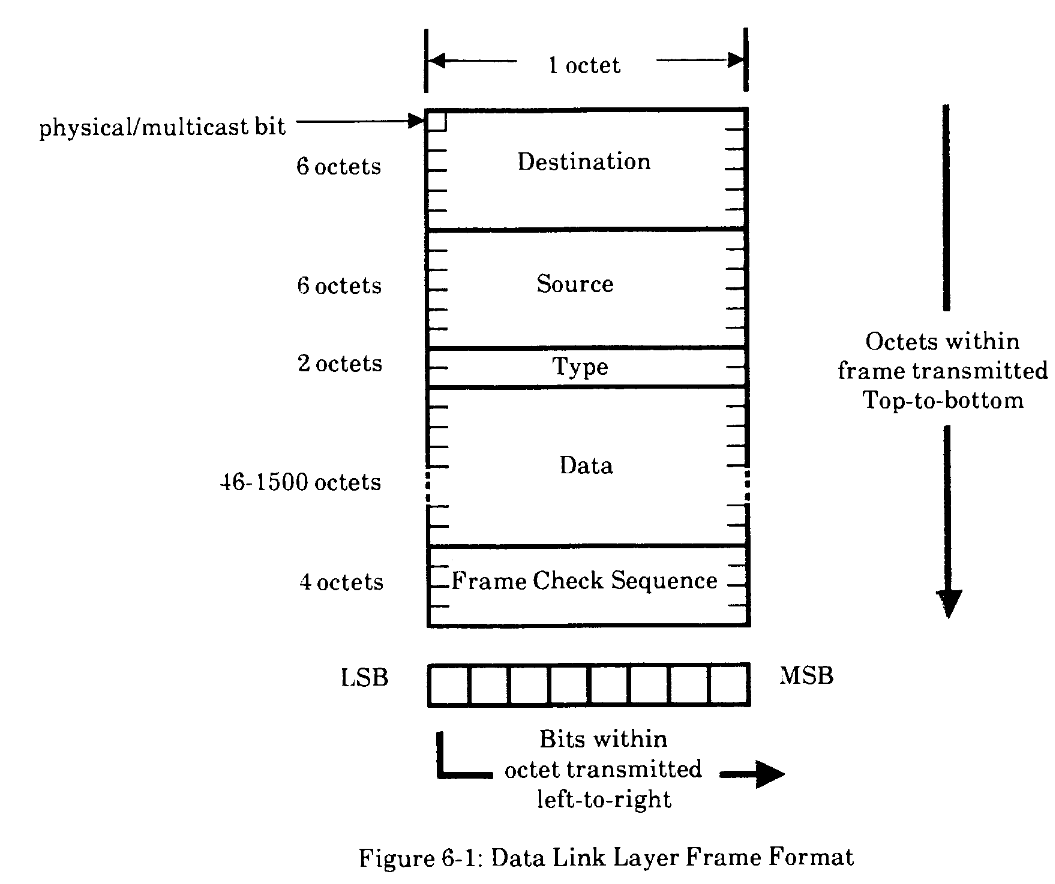
\includegraphics[height=0.85\textheight,trim={6cm 0 0 0},clip]{../buses/ether-frame}
};
\draw[red,very thick] ([xshift=2.3cm,yshift=-1.1cm]ether frame.north west) rectangle ([xshift=4.9cm,yshift=-3cm]ether frame.north west);
\node[anchor=north west,align=left] at (ether frame.north east) {
    messages needs a `\myemph{header}' to tell \\ who it's to/from \\ ~ \\
    everyone needs to filter out messages \\ that aren't theirs
};
\end{tikzpicture}
\imagecredit{Figure from Digital, Intel, and Xerox, ``The Ethernet: A Local Area Network: Data Link Layer and Physical Layer Specification'', Version 2.0 (1982)}
\end{frame}

\begin{frame}{taking turns on shared bus?}
    \begin{itemize}
    \item token ring
        \begin{itemize}
        \item one machine has a `token' = can send
        \item send special message to pass to another machine
        \end{itemize}
    \item free-for-all: collision detection + retry
        \begin{itemize}
        \item detect if you're transmitting when someone else is
        \item wait (usually randomized amount of time) and retry
        \end{itemize}
    \item coordinating machine transmits timeslots
        \begin{itemize}
        \item part of common cellphone design (TDMA: time division multiple access)
        \end{itemize}
    \item make bus support multiple transmitters?
        \begin{itemize}
        \item requires understanding how interference works
        \item another part of common cell phone design
        \end{itemize}
    \end{itemize}
\end{frame}

\againframe<5>{connectingThings}

\begin{frame}{what does the hub do?}
    \begin{itemize}
    \item simple version:
        \begin{itemize}
        \item imitate shared bus: copy messages to everyone else
        \item something to handle two messages sent at once
        \end{itemize}
    \item less simple:
        \begin{itemize}
        \item read ``header'' on message + send to destination only
        \item requires some way to figure out destinations
        \item queue of messages waiting to be sent
        \end{itemize}
    \end{itemize}
\end{frame}

\againframe<6>{connectingThings}

\begin{frame}{more complicated designs}
    \begin{itemize}
    \item hierarchies
    \item networks of networks
        \begin{itemize}
        \item ``internetworks''
        \end{itemize}
    \item so far still have single points of failure
    \end{itemize}
\end{frame}

\againframe<7>{connectingThings}
